Modern scientific discoveries and business intelligence rely heavily on large-scale simulation and data analytics. The next generation of parallel applications will require massive computing capacity to support the execution of predictive models and analysis of massive quantities of data, with significantly higher resolution and fidelity than what is possible within existing computing infrastructures. In order to deliver the desired performance of emerging  applications, future HPC and Cloud computing infrastructure is expected to continue to grow in both scale and complexity, resulting in an urgent need for efficient and scalable fault tolerance solutions to all kind of causes and symptoms. 

A significant body of work targets at improving the scalability of checkpoint/restart, while also lots of efforts are devoted to making process replication based approaches a viable alternative. Most of the existing work assumes a fail-stop fault model, such that failures are detectable by monitoring hardware or network. Silent data corruption (SDC) is yet a another class of failures. Different from crash failures, SDC may remain undetected and corrupt the intermediate or final results. It materializes as bit flips in storage (both volatile and non-volatile memory) or even within processing cores. In modern computers, a single bit flip in memory can be detected with cyclic redundancy check (CRC) and corrected with error correction code (ECC). Double bit flips, however, is beyond the hardware fault tolerance capability in most systems. Meanwhile, even single bit flips in the processor core remain undetected as only caches feature ECC while register files or even ALUs typically do not~\cite{fiala_2012_sdc}.



In large-scale production systems, SDC has become a major concern for the user, which can not only cause data loss, but also has serious impact on the integrity of job outputs, jeopardizing scientific research or business decisions. 
SDC is one of the most critical problems in cloud data processing~\cite{wang2015understanding}. 
As the capacity of and memory and disks grows, the likelihood of SDC caused by hardware failures also increases. For example, a hard drive failure resulted in Facebook temporarily losing over 10\% of photos published on their social network~\cite{wang2015understanding}. Similarly, SDC due to software bugs also becomes prevalent as the scale of cloud systems keeps expanding. For example, Amazon Simple Storage Service (S3) once experienced a data corruption problem caused by a load balancer bug~\cite{balding2009question}. In HPC systems, SDC is also attracting more attention. It is reported that, due to the high density of DIMMs, Cray XT5 at Oak Ridge National Lab’s encounters double bit flips on a daily basis~\cite{geist2011monster}. Although previous studies  have shown that disk errors and DRAM errors in large-scale production systems are happening often enough to require attention, little research has been done to answer to this challenge~\cite{fiala_2012_sdc}.

This chapter applies the Leaping Shadows model, discussed in Chapter~\ref{chapter:scale}, to deal with SDC in large-scale computing systems. In order to detect and correct SDC, we come up with a new scheme that equips Leaping Shadows with triple modular redundancy, similar to \cite{fiala_2012_sdc}. This new scheme inherits the adaptivity and power-awareness from Leaping Shadows, and optimizes a combination of process execution rates to balance the trade-offs among time, hardware, and power. In the following sections, we first describe a parallel programming paradigm typically used in compute- and data-intensive applications. Next, we
present the new Leaping Shadows scheme with its execution model. Then we build analytical models to study its performance and power requirements, and form an optimization framework, which derive the optimal execution parameters. Lastly, comparative analysis and evaluation results are given.  

%HPC and Cloud are two ecosystems that are designed for different applications and with disparate design principles. However, Big data technologies, such as Hadoop, clustered storage, and data visualization, are now merging with traditional HPC technologies. On the one hand, an increasing portion of HPC workloads is becoming data intensive. On the other hand, Big data applications are requiring more and more computing power. As the boundaries between Cloud and HPC continue to blur, it is clear that there is an urgent demand for a systematic computational model that adapts to the computing platform and accommodates the underlying workloads. 

%Recognizing this challenge, we study Leaping Shadows as a systematic computational model, that achieves power-aware fault tolerance for both compute- and data-intensive applications. In chapter~\ref{chapter:scale}, we discuss the application of the Leaping Shadows model to compute-intensive workloads in HPC, in which communication and synchronization may be frequent. Analytical models and evaluation demonstrate that Leaping Shadows can achieve higher performance and significant energy savings in comparison to existing approaches in most cases. This chapter focuses on data-intensive applications in the Cloud.

\section{Parallel Programming Paradigm}

Parallel computing frameworks, such as MPI, MapReduce, and Pregel, have been widely adopted for large-scale data analytics and simulation. To efficiently handle the sheer amount of data, and to utilize a cluster of nodes and/or multiple processors within a node, these frameworks typically arrange a job into hundreds or thousands of tasks scheduled to execute in parallel.
There are two widely adopted approaches to parallelism.
In task-parallelism, we partition the various tasks carried out in solving the problem among the processors. In data-parallelism, we partition the data used in solving the problem among the processors, and each processor carries out more or less similar operations on its part of the data. Despite the parallelism approach, the parallel processing paradigm is abstracted by the Bulk Synchronous Parallel (BSP) model~\cite{skillicorn1997questions}. 
%, each processing one partition of the whole dataset\footnote{For iterative and graph algorithms, multiple stages of such parallel execution may be needed.}. This paradigm is depicted in Figure~\ref{fig:bsp}.



According to the BSP model, there is a set of processors which may follow different threads of computation, with each processor equipped with fast local memory and interconnected by a communication network. A BSP computation proceeds in a series of global supersteps, which consists of three components:
\begin{itemize}
	\item Computation: every participating processor may perform local computations, i.e., each process can only make use of values stored in the local fast memory of the processor. 
    \item Communication: The processes exchange data between themselves to facilitate remote data storage capabilities.
	\item Barrier synchronization: When a process reaches this point (the barrier), it waits until all other processes have reached the same barrier.
\end{itemize}
%This is depicted in Figure~\ref{fig:bsp}. 
Pregel is directly inspired by the BSP model. 
In MPI programs, whose main body usually consists of a loop, each iteration could be a BSP superstep. This is also true for iterative MapReduce applications, in which each superstep includes a map or a reduce phase. 


%\begin{figure}[!h]
%  \begin{center}
%      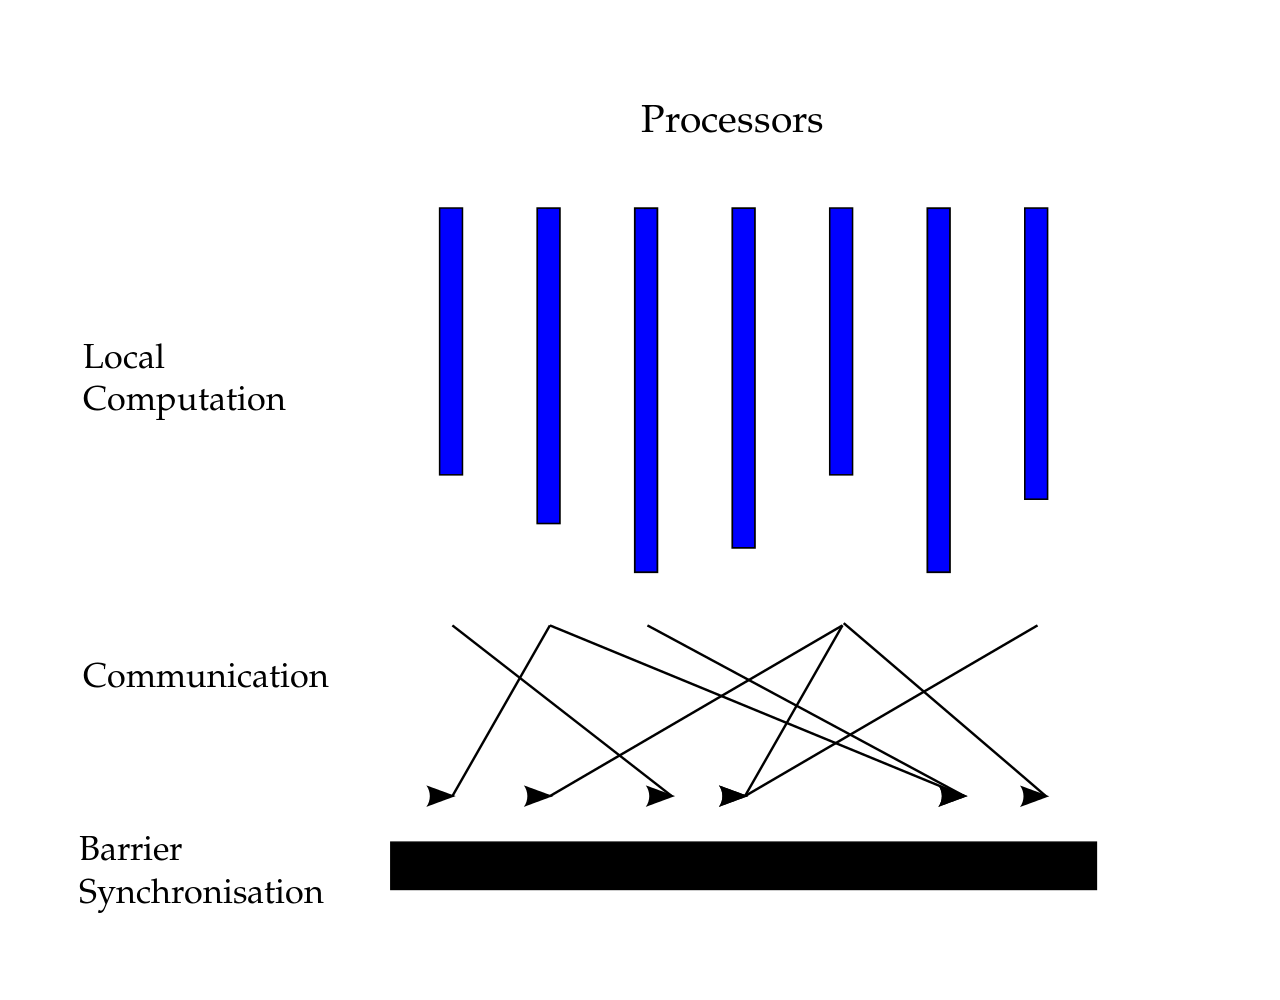
\includegraphics[width=0.8\columnwidth]{Figures/bsp}
%  \end{center}
%  \caption{Bulk synchronous parallel processing paradigm.}
%  \label{fig:bsp}
%\end{figure}

In today's parallel computing frameworks, re-execution on top of a heartbeat protocol is mainly used to provide fault tolerance and to deal with staggers. This approach works fine for system scales such that failures are rare and applications that are delay-tolerant. If failures are frequent, however, large delay can be incurred since one faulty task or stagger may delay the whole job execution. In addition, re-execution only handles crash failures. This is not acceptable for applications with strict response time requirements or applications that are vulnerable to SDC. In contrast, Leaping Shadows, if applied, will enable these frameworks to trade-off among multiple objectives, while respecting any hard or soft deadline and handling both crash failures and SDC. 

\section{Leaping Shadows Execution Model}
%\section{Dealing with silent data corruption}
Different from crash failures which crash a processor, silent data corruption allows a faulty processor to continue to completion but may silently generate incorrect results. To deal with $f$ failures, $(2f+1)$ replicas are needed, and voting is required periodically to detect failure. For example, when at most 1 silent data corruption could occur, 3 replicas are sufficient to detect and tolerate the failure. In the following, we will focus on tolerating one silent data corruption per task. 

Compared to traditional replication techniques, Leaping Shadows can deal with silent data corruption with higher efficiency and less resource requirement. For each task, Leaping Shadows associates two shadows with each main process. One shadow is designated as the primary shadow, and its duty is to compare with its associated main at a voting point to detect SDC. Based on the BSP model, each barrier synchronization is naturally a voting point. In order to detect failure as soon as possible,
the primary shadow executes at the same rate as its associated main. In addition to a primary shadow, a secondary shadow is needed to correct a SDC, once occurred, through voting. 
To save energy, the secondary shadow executes at a potentially lower rate than the other two replicas, and dynamically speeds up if failure is detected. 

To take advantage of the forward progress of the fast replicas, Leaping Shadows performs a leaping at every voting point to leap forward the secondary shadow when possible. Specifically, when the main and the primary shadow both arrive at a voting point and they reach  agreement, the results and execution state are copied to the secondary shadow to achieve forward progress. This is illustrated in Figure~\ref{fig:silent_model}. Since this leaping is triggered by a voting, it is referred to as \textit{voting-induced leaping}. If the main or the primary shadow experiences a SDC, the failure will be detected at the next voting point. At this time, the secondary shadow speeds up to reach the specific voting point, and participates in the voting to detect which replica fails. Then a leaping from one correct replica to the failed replica can rejuvenate the failed one, after which all replicas resume normal execution. Note that the secondary shadow is only useful when one of the other two replicas fails. If the secondary shadow fails, it will automatically get rejuvenated by leaping. 

\begin{figure}[!h]
  \begin{center}
      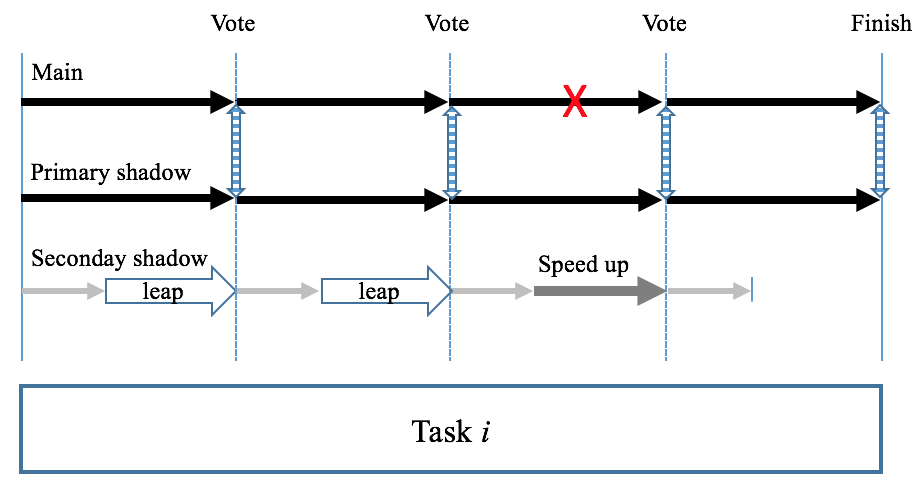
\includegraphics[width=0.8\columnwidth]{Figures/silent_model}
  \end{center}
  \caption{Tolerating SDC by applying Leaping Shadows with triple modular redundancy.}
  \label{fig:silent_model}
\end{figure}


\section{Analytical Models and Optimization Framework}
To assess the efficiency of Leaping Shadows to deal with SDC, following subsections develop analytical models for the expected response time and energy consumption under a failure distribution. Then using these analytical models, an optimization problem is formulated to minimize the expected energy consumption of Leaping Shadows under strict deadline constraint. This not only demonstrates Leaping Shadows' adaptivity to the desired trade-off, but also provides a framework with which we can perform comparative performance analysis to state-of-the-art approaches.

\subsection{Notations}
Let $W$ denote the total workload to process a task. Let $N$ denote the number of BSP supersteps, which is also the number of voting points. Then each voting interval has a workload of $w=\frac{W}{N}$. Let $\sigma_{max}$ denote the maximum execution rate. $R_{min}=\frac{W}{\sigma_{max}}$ is the minimal response time. Let $\overline{R}=(1+\alpha)R_{min}$ $(0\leq \alpha \leq 1)$, where $\alpha$ is called laxity factor, denote the target response time considering fault tolerance overhead. Let $\lambda$ denote the failure rate, and $f(t)$ denote the failure density function. %Let $d(t)$ denote the failure detection time at a voting point. 
Let $E(\sigma, [t_1, t_2])$ denote the energy consumption of a replica when executing at rate $\sigma$ for an interval from $t_1$ to $t_2$. For each leaping, let $T_l$ denote the time overhead, and $E_l$ denote the energy cost.

To deal with silent data corruption, the Leaping Shadows model associates two shadows with the main process for each task. According to the execution model described in above section, there are three execution rates:
\begin{itemize}
	\item $\sigma_m$, the execution rate of the main and the primary shadow 
    \item $\sigma_b$, the execution rate of the secondary shadow before a SDC is detected 
    \item $\sigma_a$, the execution rate of the secondary shadow after a SDC is detected 
\end{itemize}

\subsection{Response Time}
Assuming there is at most one silent data corruption per task, two scenarios need to be considered, i.e., a SDC occurs to the main process or the primary shadow, or neither of them fails. The failure of the secondary shadow has no impact on the response time, thus is ignored in the following analysis. 

In the first scenario, where no failure occurs, the execution time is determined by the main process, as $t_r^m=\frac{W}{\sigma_m}$. Considering the time for leaping, the total response time is $t_{rl}^m=\frac{W}{\sigma_m} + N \times T_l$.

In the second scenario, 
where a fast replica fails, the delay is the time for the secondary shadow to catch up with respect to a voting interval. The time for the main process to complete a voting interval is $t_v = \frac{w}{\sigma_m}$. The time required by the secondary shadow to complete the remaining work in the current interval is $t_d = \frac{w - t_v\times \sigma_b}{\sigma_a}$. The execution time is $t_r^s = t_r^m + t_d$. Considering the time for leaping, the total response time is $t_{rl}^s=t_r^s + N \times T_l$.


\subsection{Power and Energy Consumption}

Dynamic voltage and frequency scaling
(DVFS) is assumed in this work to achieve the desired execution rate of a process. It
is well known that one can reduce the dynamic processor power consumption at
least quadratically by reducing the frequency linearly. The
dynamic processor power consumption executing at rate
$\sigma$ is given by the function $p_d(\sigma)=\sigma^n$ where $n \ge
2$. Throughout this section, we assume that dynamic power is cubic in relation to the processor frequency.

In addition to the dynamic power, processor leakage and other components
(memory, disk, network etc.) all contribute to static power
consumption, which is independent of the processor frequency. In this section, we
define static power as a fixed fraction of the total power consumed
when executing at maximum rate, referred to as $\rho$. Hence, a processor's
power consumption is expressed as
$p(\sigma)=\rho \times \sigma_{max}^3 + (1-\rho)\times \sigma^3$.

Next we calculate the expected energy consumption for a single task under Leaping Shadows. 
Corresponding to the two scenarios in the above response time analysis, the energy consumption also falls into two cases. 
If neither of the main process and primary shadow fails, the energy consumption of the three replicas weighted by its probability is
\begin{equation}
%\begin{split}
E_1 =  (1 - \int_{0}^{t_r^m} f(t)dt)^2  \times 
       \{2E(\sigma_m, [0, t_r^m])+E(\sigma_b, [0, t_r^m])\}
%E_1 = & (1 - \int_{0}^{t_r^m} f_m(t)dt)^2  \times \\
%      & \{2E(\sigma_m, [0, t_r^m])+E(\sigma_b, [0, t_r^m])\}
%\end{split}
\end{equation}
The first factor is the probability that neither of them fails, as $\int_{0}^{t_r^m} f(t)dt$ is the probability that a replica encounters a SDC during task execution. The second factor models the energy of the three replicas from task start to end, with two replicas executing at rate $\sigma_m$ and one replica executing at $\sigma_b$.

If the main or the primary shadow fails, the energy consumption weighted by its probability is 
\begin{equation}
\begin{split}
E_2 = & 2 \times (1 - \int_{0}^{t_r^m} f(t)dt) \times \int_{0}^{t_r^m} f(t)dt \times 
\\  & \{2E(\sigma_m, [0, t_r^m])+E(\sigma_b, [0, t_r^m])  + 2E(0, [t_r^m, t_r^s])+E(\sigma_a, [t_r^m, t_r^s]\} 
%E_2 = & 2(1 - \int_{0}^{t_r^m} f_m(t)dt) \times \int_{0}^{t_r^m} f_m(t)dt \times 
%\\  & \{2E(\sigma_m, [0, t_r^m])+E(\sigma_b, [0, t_r^m]) \\ & + 2E(0, [t_r^m, t_r^s])+E(\sigma_a, [t_r^m, t_r^s]\} 
\end{split}
\end{equation}
The first line calculates the probability that one fast replica fails while the other successfully completes. In addition to the energy in the first scenario, also accounted is the energy consumed during the secondary shadow catches up. This energy corresponds to the main process and the primary shadow idly waiting and the secondary shadow speeding up to reach the next voting point. 



All in all, the total energy consumption is the sum of the above two, plus the energy cost of leaping, i.e., $E_{total}=E_1 + E_2 + N\times E_l$. 

\subsection{Optimization}
\label{sec:silent_opt}
When applying Leaping Shadows to deal with SDC, an optimization problem formulation is also needed to derive the optimal execution rates for both the main and shadow processes. With the generic optimization framework introduced in Chapter~\ref{chapter:shadowing}, we define the optimization objective as minimizing energy under response time constraint:

\begin{equation}
\begin{alignedat}{2}
\min_{\sigma_m,\sigma_b,\sigma_a} \qquad  & E_{total} (W,N,\overline{R},\rho,\lambda,\sigma_{max}, T_l, E_l)  \\
s.t.  \qquad          & 0 \leq \sigma_m \leq \sigma_{max} \\
                      & 0 \leq \sigma_b \leq \sigma_m\\
                      & \sigma_b \leq \sigma_a \leq \sigma_{max} \\
                      & t_{rl}^s \leq \overline{R}
\end{alignedat}
\end{equation}



The first constraint says the execution rate of the main process and primary shadow should observe the physical processor limit. The second constraint indicates that the initial rate of the secondary shadow should not exceed that of the main process and primary shadow. The third constraint ensures that the secondary shadow could speed up after detecting a failure. The last constraint guarantees that the deadline is met even in the case of failure. Same as before, non-linear optimization techniques can be used to solve the above problem, and the output will be the three optimal execution rates.

\section{Evaluation}
Using the optimization framework developed above, this section evaluates the performance of Leaping Shadows by comparing with traditional process replication using triple modular redundancy~\cite{fiala_2012_sdc}, under various environments and different application requirements. With an uniform treatment of the replicas, process replication requires all three replicas execute at the same rate before and after a failure. In the comparison, however, we also optimize this single rate for process replication in a way similar to Section~\ref{sec:silent_opt}\footnote{Process replication is a special case of Leaping Shadows where $\sigma_m = \sigma_b = \sigma_a$.}, in order to demonstrate the benefits of the unique design in Leaping Shadows. 

After careful analysis of the analytical models, we identify the important parameters of static power ratio, laxity in deadline, workload, number of voting interval, and leaping cost, and study the impact of each parameter. With the understanding that failure rate of each processor will remain more or less the same in the near future, We fix MTBF to be 5 years for realistic consideration. %Also, because workload does not change the energy consumption as in above subsection, we do not show its study and instead fix it to be 100 hours per processor. 
The comparison results are shown in Figure~\ref{fig:silent_eval}.

\afterpage{
\begin{figure}[!t]
	\begin{center}
		\subfigure[Impact of static power ratio. $\alpha=50\%$, $N=10$, $W=100$ hours.]
		{
			\label{fig:silent_power}
			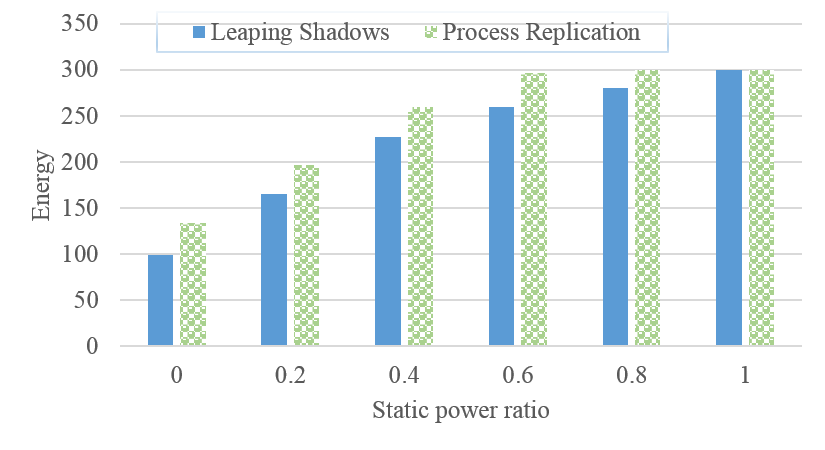
\includegraphics[width=0.45\textwidth]{Figures/silent_power}
		}
		\subfigure[Impact of laxity. $\rho=0.3$, $N=10$, $W=100$ hours.]
		{
			\label{fig:silent_laxity}
			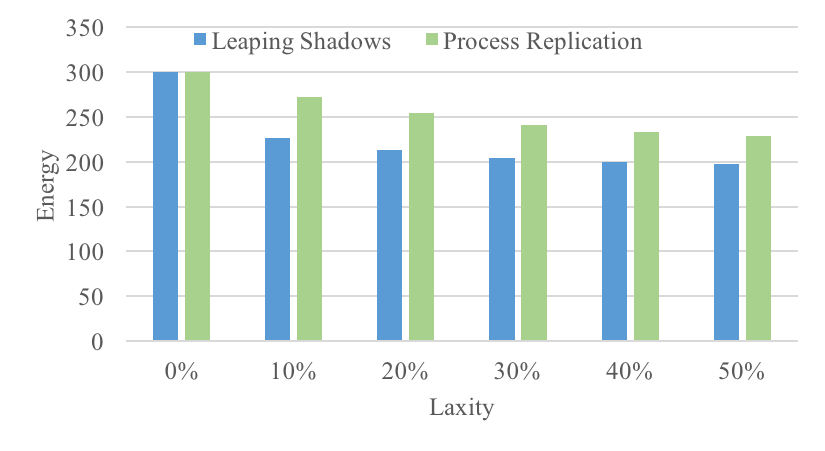
\includegraphics[width=0.45\textwidth]{Figures/silent_laxity}
		}
        \vskip 0.5in
        \subfigure[Impact of voting interval. $\alpha=50\%$, $\rho=0.5$, $W=100$ hours.]
		{
			\label{fig:silent_interval_1}
			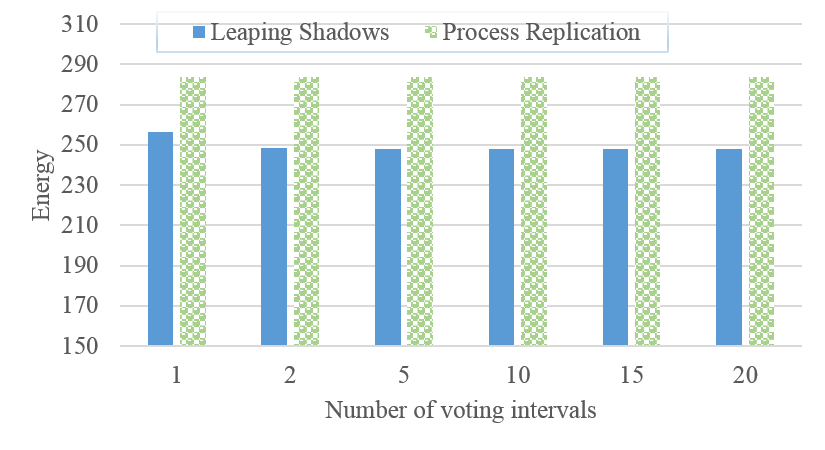
\includegraphics[width=0.45\textwidth]{Figures/silent_interval_1}
		}
        \subfigure[Impact of voting interval. $\alpha=50\%$, $\rho=0.3$, $W=100$ hours.]
		{
			\label{fig:silent_interval_2}
			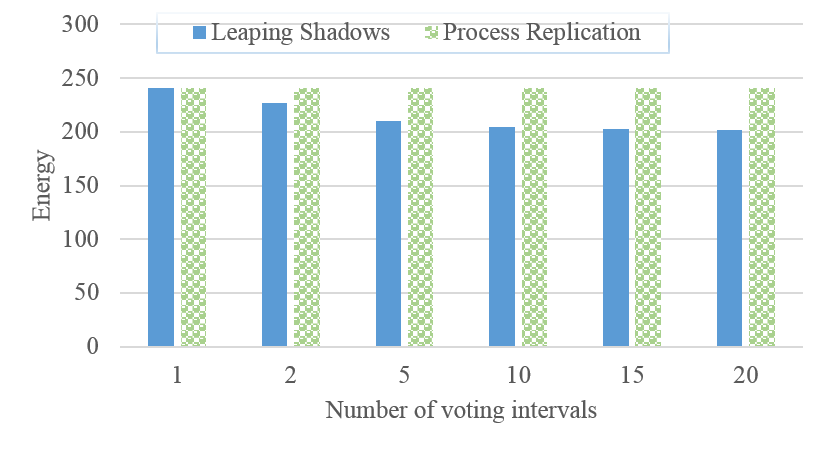
\includegraphics[width=0.45\textwidth]{Figures/silent_interval_2}
		}
        \vskip 0.5in
        \subfigure[Impact of task workload. $\alpha=25\%$, $\rho=0.5$, $N=10$.]
		{
			\label{fig:silent_workload}
			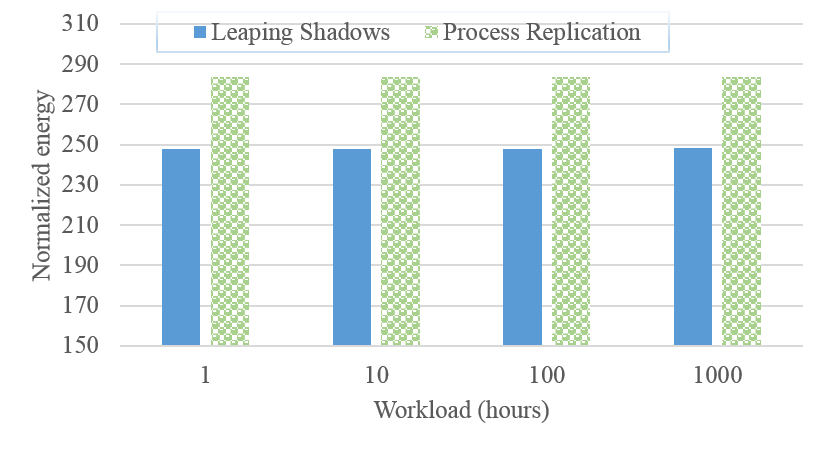
\includegraphics[width=0.45\textwidth]{Figures/silent_workload}
		}
        \subfigure[Impact of leaping cost. $\alpha=50\%$, $\rho=0.5$, $N=10$, $W=100$ hours.]
		{
			\label{fig:silent_leap}
			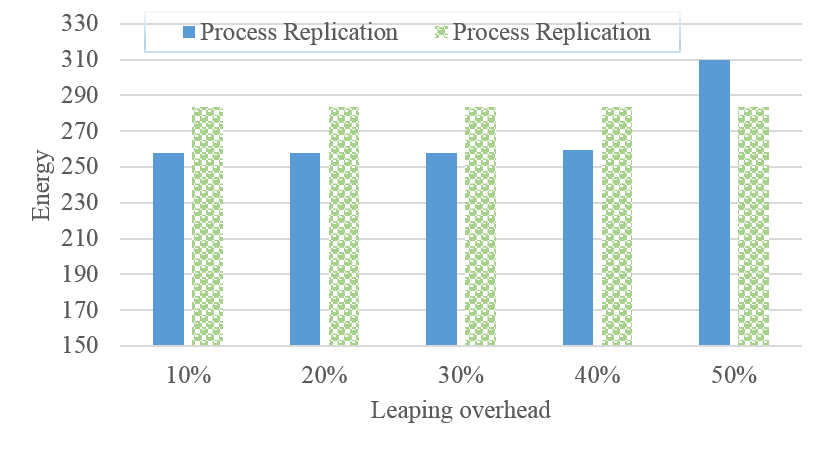
\includegraphics[width=0.45\textwidth]{Figures/silent_leap}
		}
	\end{center}
	\caption{Comparison between Leaping Shadows and process replication for energy consumption under silent data corruption. MTBF=5 years.}
	\label{fig:silent_eval}
\end{figure}

\clearpage
}

Figure~\ref{fig:silent_power} reveals the energy consumption of the two compared approaches at different static power ratios, when laxity is 50\% and number of voting intervals is 10. When static power ratio is less than 0.8, both approaches reduces the execution rates to minimize energy. At 0 static power ratio, Leaping Shadows saves 25.6\% energy compared to process replication. The saving decreases as static power ratio increases, and finally Leaping Shadows converges to process replication when static power ratio reaches 1. Modern computers has a static power ratio between 40\% and 70\%~\cite{butts2000static}. Within this target range of static power ratio, Leaping Shadows achieves 12.5\% energy savings with respect to process replication.
%Note that energy saving is less than that of crash failure tolerance because both fast and slow replicas have to process a partition from the same end in order to detect and tolerate silent data corruption.

With 10 voting intervals and 0.3 as the static power ratio, the impact of laxity is illustrated in Figure~\ref{fig:silent_laxity}. When there is no laxity, Leaping Shadows is forced to execute all three replicas at the maximum rate, which is essentially process replication. As laxity increases, both compared approaches have more room to slow down, thereby reducing energy. By coupling two fast replicas with a slow one and using leaping to achieve forward progress for the slow replica, Leaping Shadows always saves 13.5\%-16.9\% energy compared to process replication when there is laxity.

One interesting questions is how the number of voting intervals changes the picture. Without considering the overhead of leaping, intuition tells us that the more voting intervals, the less effect a failure can have on the total execution time of Leaping Shadows, and thus the better performance. This is mostly true, according to Figure~\ref{fig:silent_interval_1}. However, the figure also shows that after the number of voting intervals reaches 5, its impact becomes negligible. We also study this behavior with static power ratio changed to 0.3, as shown in Figure~\ref{fig:silent_interval_2}. 
As a result, both of the two compared approaches are able to reduce energy consumption by further slowing down. 
Although the difference between them decreases at a small number of voting intervals, Leaping Shadows keeps increasing its energy savings with the number of voting intervals, up to 20.

The next parameter studied is the total workload, which determines the failure-free execution time, and thus the propensity of the task to failures. For Figure~\ref{fig:silent_workload}, we vary the task workload from 1 hour to 1000 hours. Compared to the 5 years' MTBF, all the workloads considered are relatively small, thus the failure of a given task is very unlikely. Therefore, there is only slight change in the energy consumption. 

All the above experiments ignore the overhead of leaping. Assuming each time leaping consumes 1 unit of energy, the last experiment studies the impact of leaping overhead, which is defined as a fraction of the minimum response time. Figure~\ref{fig:silent_leap} reveals that when the overhead is below 30\%, it has negligible impact. At 40\% overhead, Leaping Shadows is forced to slightly increase its rates, and thus incurs a slightly higher energy consumption. When overhead is 50\%, it essentially offsets the laxity, which is 50\%, and leaves no room for Leaping Shadows to slow down. As a result, all replicas need to execute at the maximum rate and end up with consuming more energy than process replication, which does not perform leaping at all.

\section{Summary}
Scientific research and engineering development are increasingly relying on computational modeling, simulation, and data analytics to augment theoretical analysis. Behind the wheel, data has become the ultimate driving force that yields insights and propels innovation. With a torrent of data generated every second from distributed sensors, social media, software logs and so on, it is critical to analyze and visualize the data in a timely manner,  at massively parallel scale, and with fault tolerance capabilities. 

Leaping Shadows is a novel fault-tolerant computational model that unifies HPC and Big Data analytics. 
The flexibility within the model allows it to embrace different optimization techniques in accordance with the underlying workloads, whether compute-intensive or data-intensive. 
By designing the execution model of Leaping Shadows in accordance with the generic Bulk Synchronous Parallel model, Leaping Shadows can be applied to both HPC and Cloud environments, to deal with different types of failures, or multiple types of failures at the same time. 

While previous chapters discuss on tolerance of crash failures, this chapter extends the Leaping Shadows model and studies the tolerance of silent data corruption. 
By exploring the interplay between performance, fault-tolerance, and energy consumption, Leaping Shadows is predicted to save a significant amount of energy (up to 64.9\%) compared to existing fault tolerance approaches, while respecting strict response time requirements. In the future, we plan to implement this model and perform intensive empirical evaluation to verify the accuracy of the analytical models.     









